\documentclass[12pt,a4paper]{report}

\usepackage{graphics}
%\usepackage{fullpage,epsf,graphicx, amstext,url} 
%\usepackage{epsf}
\usepackage{graphicx}
\usepackage{amstext}
\usepackage{url}
\usepackage{amssymb}
\usepackage{graphicx}
\usepackage{amsmath}

%\graphicspath{ {/home/george/Desktop/Tex_Dissertation/images} }
%
% head.sty is no longer needed
%
%\usepackage{head,fullpage,epsf,graphicx, amstext,url} 

\def\BibTeX{{\rm B\kern-.05em{\sc i\kern-.025em b}\kern-.08em
    T\kern-.1667em\lower.7ex\hbox{E}\kern-.125emX}}

\begin{document}

\thispagestyle{empty}

%                       This is a basic LaTeX Template
%                       for the MSc Dissertation report
%
\parindent=10pt          %  Switch off indent of paragraphs 
\parskip=5pt            %  Put 5pt between each paragraph  
%
%                       This section generates a title page
%                       Edit only the sections indicated to put
%                       in the project title, and submission date
%

\vspace*{0.1\textheight}

\begin{center}
        \huge{\bfseries Calculation of the Supersymmetric top quark mass at CLIC}\\
\end{center}

\bigskip

\begin{center}
        \large{Georgios Billis}\\      % Replace with your name
        \bigskip
        \large{August 18, 2017}        % Submission Date
\end{center}

%%% If necessary, reduce the number 0.4 below so the University Crest
%%% and the words below it fit on the page.
%%% Don't let the crest and the wording below it flow onto the next page!
\vspace*{0.35\textheight}

\begin{center}
        
\includegraphics[width=35mm]{crest.pdf}
\end{center}

\medskip

\begin{center}

%%%
%%% Change Theoretical to Mathematical if appropriate
%%%
\large{
  MSc in Theoretical Physics\\[0.8ex]
  The University of Edinburgh\\[0.8ex]
  2017
}

\end{center}

\newpage


\pagenumbering{roman}

\begin{abstract}
In this project I calculate the mass of the Supersymmetric top quark in CLIC experiment at $\sqrt{s}$ = 3 TeV in $e^{-}$ $e^{+}$ collisions. I assume the following decay for the top squark $\tilde{q} \rightarrow q$ $\chi_{0}$, 
and I focus on the fully hadronic channel of decay i.e $\tilde{q} \rightarrow q$ $\chi_{0} \rightarrow$ $W b \tilde{\chi}_{1}^{0}$ .
The mass was found  to be  $m_{\tilde{t}}$ = 861 $\pm$ 19 GeV using the Boosted Descision 
Trees Multivariate Analysis and $m_{\tilde{t}}$ = 812 $\pm$ 20 GeV using the Gradient Boosted Descision  Trees Multivariate Analysis. 
\end{abstract}

\pagenumbering{roman}


\textbf{Declaration}


\newpage

\tableofcontents
\listoftables
\listoffigures

\begin{titlepage}
\vspace*{2in}
% an acknowledgements section is completely optional but if you decide
% not to include it you should still include an empty {titlepage}
% environment as this initialises things like section and page numbering.
\section*{Acknowledgements}

Put your acknowledgements here. Thanking your supervisor for his/her
help is standard practice, but you don't have to do this\ldots

This template is is modification of the one for the MSc in High
Performance Computing, which is apparently descended from a template
developed by Prof Charles Duncan for MSc students in Meteorology. His
acknowledgement follows:

\emph{This template has been produced with help from many former
  students who have shown different ways of doing things. Please make
  suggestions for further improvements.}

Some parts of this template were lifted unashamedly from the Edinburgh
MPhys project report guide, with little or no modification. I have no
idea who wrote the first version of that\ldots

You don't have to use \LaTeX\ for your dissertation. You can use
Microsoft Word or Apple Pages if you wish, but it's \emph{much} easier
to typeset equations in \LaTeX, and references look after
themselves. Whatever you use, your dissertation should have the same
general structure, and it should look similar to this one --
especially the front page.


\end{titlepage}

\pagenumbering{arabic}

\chapter{Introduction}

On July 2012 the discovery of the Higgs boson was announced at CERN's Large Hadron Collider (LHC). This marked the begining of a new era for experimental High Energy Physics motivating the design of new 
experiments for further and deeper exploration of the Higgs boson itself but also, a huge marathon
addressing the questions/problems that arose with it. 

One of these proposed experiments is Compact Linear Collider (CLIC), a high-luminosity linear $e^{-}$ $e^{+}$ collider. It is designed for a staging scenario of three main centre of mass energies at $\surd{s}$ = 380 GeV, $\surd{s}$ = 1.5 TeV
and $\surd{s}$ = 3 TeV targeting optimal physics output based on the current landscape. The main difference of CLIC with LHC is that in the latter, protons collide which are non fundamental particles as they consist of quarks and 
gluons bound alltogether. One of the disadvantages of LHC is the inability to know beforehand the initial state of the colliding particles as quarks exist in a "sea of gluons" making it impossible to know their momenta. This sets
some restrictions with resprect to the precision that it can probe various observables.

On the other hand, CLIC is designed to invastigate the interactions of elementary particles, an important advantage since initial states of the colliding particles is known. In advance, LHC suffers from energy loss due to 
Synchrotron radiation since protons are accelerated in a 27 km circular accelerator whereas CLIC, being linear does not.

The main targets of CLIC are dependent of the energy stage. In the first it will focus on prescision standard model physics such as Higgs and Top quark measurements and in the two subsequent, among others, there will be searches
for new physics~\cite{clic2016updated}. One of the theories that aspires to give solutions to many of the problems of Standard Model is Supersymmetry (SUSY). In this theory every particle has a Supersymmetric partner that differs in the spin by $1/2$, thus 
relating bosons with fermions and fermions with bosons.

In the Minimal Supersymmetric Standard Model, the top squarks $\tilde{t}$ decay almost all the times into a top quark $t$
and a dark matter candidate, the neutralino $\tilde{\chi}_{1}^{0}$. In this project I will use Multivariate Analisis
to discriminate the best it can be achieved between signal and background with the goal to measure the top squark
mass at $\surd{s}$ = 3 TeV in the CLIC accelerator environment.






\chapter{CLIC}

\section{Outline of the experiment}

CLIC is a proposed $e^{-}$ $e^{+}$ linear collider optimised to perform in three centre of mass stages at 
$\surd s$ = 380 GeV, $\surd s$ = 1.5 TeV and $\surd s$ = 3 TeV. The purpose of the different energy stages is to 
fully exploit its scientific potential including precision measurements and searches for physics Beyond the 
Standar Model.

Specifically, at $\surd s$ = 380 GeV and with an integrated luminosity of $\mathcal{L}_{int}$ = 500 fb$^{-1}$, 
prescision measurements can be made in the Higgs and the top quark sector. At this enegy stage the Higgsstrahlung
process ($e^{+}e^{-}\rightarrow ZH$) alongside the $WW$ fusion ($e^{+}e^{-}\rightarrow H\nu_{e}\tilde{\nu}_{e}$) 
are the dominant and can shed light to properties of the Higgs boson in a model independent way~\cite{clic2016updated}.
In CLIC there is also a dedicated program for top quark physics, as it is one of the most important particles
in SM because it couples strongest to the Higgs field due to its mass but also it has an important role in 
many of the BSM scenarios.
Furthermore at the next two stages leading role will play the proposed scenarios for physics BSM with most 
importantly Supersymmetry at $\surd s$ = 3 TeV and with $\mathcal{L}_{int}$ = 2000 fb$^{-1}$. This  is because CLIC has the potential for direct particle detection up to the 
kinematic limit of $\surd s /2$ for pair production but also through indirect detection of observables that are sensitive to BSM
scenarios through precision measurements and comparison with the SM expectations, 
taking advantage of the full energy potential.



Given the linear nature of CLIC, there are no energy losses induced by Synchrotron radiation which appears in 
circular colliders, but due Beamsstrahlung radiation. As the colsliding bunches get closer to the 
vertex, the strong electromagnetic fields (up to 10 Tesla) created by the opposing beam, cause deflection
of the partices trajectories resulting to emit Synchrotron radiation. The effect is energy-dependent with huge
impact at higher energies~\cite{bonvicini1989first} as it can be seen in the following 
image~\cite{abramowicz2017higgs}.

\begin{figure}[h!]
  \centering
  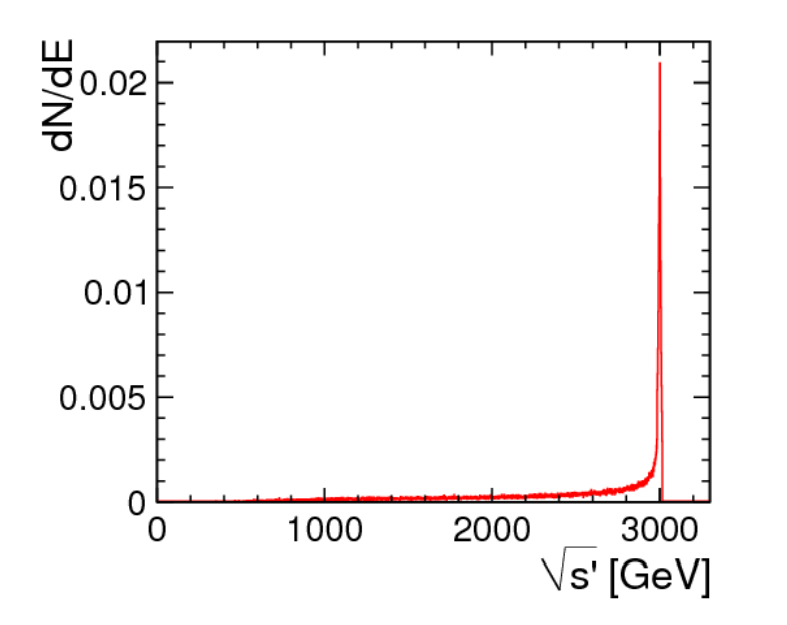
\includegraphics[width=0.7\linewidth]{{images/beamsstrahlung}.png}
  \caption{The luminosity spectrum for CLIC operating at $\surd s$ = 3 TeV, where $\surd s'$ is the
  effective centre-of-mass energy after beamstrahlung and initial state radiation }
  \label{fig2.15}
\end{figure}

CLIC is designed to operate for seven, five and six years respectively in each energy stage while the 
upgrading periods will last two years. The total run will last for 22 years with the following table summarising
the luminosities achieved in each stage:

\begin{table}[h]

\centering % used for centering table
\begin{tabular}{c c} % centered columns (4 columns)
\hline %inserts double horizontal lines
$\surd s$ (GeV)  & $\mathcal{L}$   \\ \hline % inserts single horizontal line
380 & 500 fb$^{-1}$  \\
1.5 & 1.5 ab$^{-1}$ \\
3   &  2 ab$^{-1}$ 
 %inserts single line
\end{tabular}
\label{table:nonlin} % is used to refer this table in the text
\end{table}

Furthermore, the experiment has two detector concepts CLIC SiD and CLIC ILD in order to serve the required 
jet energy resolution. The latter has been  developed for the International Linear Collinder but it has been
adapted according to the needs of CLIC. Both detectors have strong central solenoid magnets creating an axial 
magnetic field of 5T for CLIC SiD and 4T for CLI ILD~\cite{abramowicz2017higgs}.



\chapter{Supersymmetry}

\section{Motivation}

The model that describes elementary particle physics is the Standar Model. It involves matter  fields (fermions)
and vector gauge bosons (force carriers) that they stem from the fact that the SM Lagrngian is subject to $SU(3) \otimes 
SU(2) \otimes U(1)$ symmetries. An important part of this theory is the existence of the Higgs field which appeared
during the unification of the electromagnetic and the weak force. It is known for the fact that it "gives"
mass to the elementary particles (besides photons and gluons which they are protected by the $U(1)$,$SU(3)$
symmetries respectively)
via Spontaneous Symmetry Breaking .

It is true that even with the great success that the SM has been probed does not consist a flawless theory.
Many parts of it are still to be answered or contain significant controversies. One example is the Hierarchy 
problem. In the electroweak sector of the SM there is a parameter that has the dimensions of energy, the 
vacum expectation value of the Higgs field which phenomenologicaly is 

\begin{equation}
 \upsilon \approx 246 \quad GeV
\end{equation}

The importance of this parameter is that it sets the masses of the the theory and as well as the Higgs boson
itself as it is

\begin{equation}
 M_{H} = \upsilon \sqrt{\frac{\lambda}{2}} 
\end{equation}


where $\lambda$ is the constant of the Higgs self interaction. The problem arises when we try compute higher 
order corrections to the mass of the Higgs field. The self energy of the higgs boson has a term of the form

\begin{equation}
 \int_{}^{\Lambda} d^{4}k \quad f(k,external\quad momenta)
\end{equation}

where $\Lambda$ represents the scale of the new physics such as the effects of quantum gravity. In dimensional 
regularisation, when $\Lambda \rightarrow \infty$ the renormalisability of the theory assures that there
is no inconsistency, but if we take into account a scale, for example, for the quantum gravity then $\Lambda \rightarrow 
M_{P} \approx 1.2\times 10^{19}\quad GeV$ which is the Plank mass, then the additive quantum corrections for the Higgs 
mass become too big dragging the value of the Higgs mass up. Because the VEV of the Higgs boson has a fixed 
phenomenologicaly value, one way to circumvent this problem is by relating bosons with fermions since in the 
latter, the algebraic terms for their self energies come with a minus sign giving the desired calcelations 
without any "fine tuning" from our side. This results into the SUSY theory stabilising the Hierarchy $M_{H}
\ll M_{P}$ with the constraint that the SUSY particles should be visible at a scale not too much greater 
than 1-10 TeV~\cite{aitchison2005supersymmetry}.

One other feature that makes SUSY attractive is the fact that it includes the convergence of the couplings,
something that it is known as Grand Unification. From the point of view of SM, something like that is 
unable to achieve since two of the couplings decrease with energy (weak and strong coupling) whereas one
(electromagnetic) increases. In the MSSM, by the inclusion of the sparticles such unification is actually
achievable as it can be seen in the following figure:

\begin{figure}[h!]
  \centering
  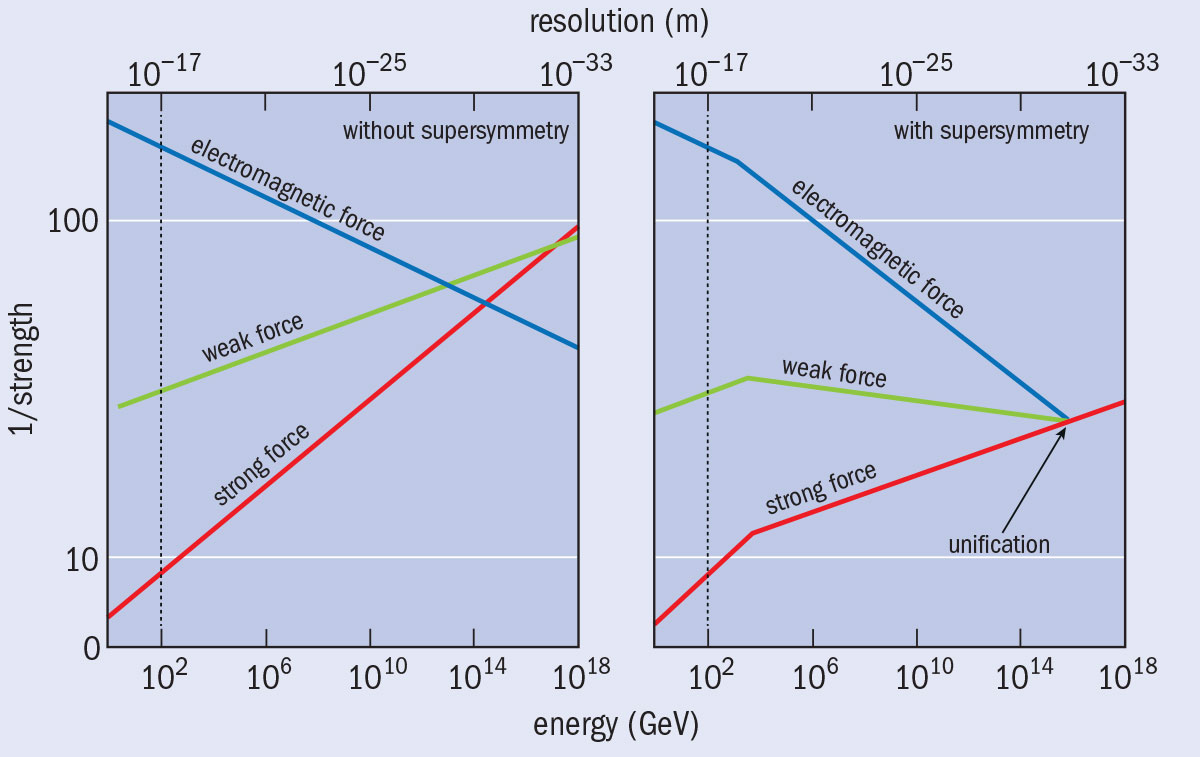
\includegraphics[width=0.7\linewidth]{{images/PWOct14gates-fig2-full}.jpg}
  \label{}
\end{figure}



\section{SUSY Phenomenology}

Inside SUSY every boson is related to a fermionic supersymmetric partner and every fermion has a bosonic one. The 
fermion superpartners are called sfermions and differ in the spin value by 1/2 whereas the boson particles 
which are the force carries are related to a spin 1/2 particles, the gauginos. In the following table I show
the correspondance between SM and SUSY gauge particles.

\begin{table}[ht]

\centering % used for centering table
\begin{tabular}{c c c c} % centered columns (4 columns)
\hline\hline %inserts double horizontal lines
Standard Model  &  & SUSY &  \\ [0.5ex] 
\hline % inserts single horizontal line
Photon & $\gamma$ & Photino & $\tilde{\gamma}$ \\ % inserting body of the table
Gluon & g & Gluino & $\tilde{g}$ \\
Z Boson & Z & Zino & $\tilde{Z}$ \\
W Boson & $W^{\pm,0}$ & Wino & $\tilde{W}^{\pm,0}$ \\
B Boson& B & Bino & $\tilde{B}$ \\ [1ex] % [1ex] adds vertical space
\hline %inserts single line
\end{tabular}
\label{table:nonlin} % is used to refer this table in the text
\end{table}

The framework of this project is the Minimal Supersymmetric Standard Model which besides the SM particles 
includes the sleptons $\tilde{\ell}^{\pm}$, the sneutrinos $\tilde{\nu}_{l}$, the squarks $\tilde{q}$, the 
gluinos $\tilde{g}$, two pair of charginos $\tilde{\chi}^{\pm}_{i}$ where $i=1,2$,  four neutralinos 
$\tilde{\chi}^{0}_{i}$, $i=1,...,4$ and five Higgs bosons $h^{0}$, $H^{0}$, $A^{0}$,$H^{\pm}$.

Both particles and sparticles belong to the same super-multiplet having the same mass and the same quantum 
numbers as their SM partners but with different spin. Because no such degenerate fermion-boson pair exists 
in nature,
then it is deduced that SUSY must be a broken symmetry. In order to constitute a solid solution to the 
Hierarchy problem, then the difference in the masses of the particles and their supersymmetric partners 
must be of the order of $\mathcal{O}(1  TeV) $~\cite{nagashima2014beyond}.

In Standard Model, for the Spontaneous Symmetry Breaking one Higgs doublet is needed with 4 degrees of 
freedom. For the SUSY model on the other hand two such doublets are required with a total of eight 
degrees of freedom where three of them are absorbed to give mass to the SM particles such as W$^{\pm}$ and Z,
and the remaining five give rise to five physical Higgs bosons $\tilde{h}$,$\tilde{H}^{\pm}$,$\tilde{A}$,
$\tilde{H}^{0}$. Those in turn, mix further to become the neutralinos and the charginos : $\tilde{\chi}_{i}^{0}$,
$\tilde{\chi}_{i}^{\pm}$. 

It is known that within the SM the fermions carry chirality denoted by L or R whether they are left or right 
respectively, according to the way they transform under the symmetry group $SU(2) \otimes U(1)$. Thus given 
the SUSY relation of fermions-bosons that means that the sfermions  (bosonic superpartners), come into 
doublets of the form $(f_{i},\tilde{f}_{i})$, where i=L,R. The sfermions mix further to make the eigenstates
of the mass matrix. This mixing is expected to be strong for third generation sfermions since the Yukawa 
couplings can be large, more precisely in our case the stop quark mixing effects can be large because
of the large mass of the top quark.

The following matrix is the mixing matrix expressed in the $(\tilde{f}_{L},\tilde{f}_{R})$ basis:

\begin{equation}
 \mathcal{M}^{2}_{\tilde{f}} =
\[  
  \begin{pmatrix}
   M^{2}_{\tilde{f}_{L}}  &  \alpha_{f}m_{f} \\
   \alpha_{f}m_{f}        &  M^{2}_{\tilde{f}_{R}}
  \end{pmatrix}
\]
\end{equation}

where the $M^{2}_{\tilde{f}_{L}}$ are terms that depend on the mass of the quark, the charge and the third 
component of the weak isospin. The off diagonal elements $\alpha_{f}$ are dependent on the soft SUSY breaking
trilinear scalar coupling parameters.

In this project I will focous on the top squarks  where the mixing   $\tilde{t}_{R}-\tilde{t}_{L}$ is important
due to the large top quark mass. By computing the eigenvalues of the previous matrix and for the right
flavour we obtain:

\begin{equation}
 m^{2}_{\tilde{t}_{1,2}} = \frac{1}{2}(M^{2}_{\tilde{t}_{L}} + M^{2}_{\tilde{t}_{R}} \mp 
 \sqrt{(M^{2}_{\tilde{t}_{L}}-M^{2}_{\tilde{t}_{R}})^{2} + 4 m^{2}_{t}\alpha^{2}_{t}})
\end{equation}

It is obvious that the $m^{2}_{\tilde{t}_{1}}$ will have the lowest mass, something that makes it the 
lightest squark.

\section{Results from LHC for SUSY}
 
 The search for indications for Supersymmetry is not new as LHC has been optimized and focused among other
 to the direct or indirect detection of sparticles. The majority of the cases that have been studied, 
 consider as main decay channel of the sparticles the following:
 
 \begin{equation}
  BR(\tilde{q} \rightarrow q  \chi_{i}^{0,\pm}) = 100 \%
 \end{equation}

So far thought no indication of SUSY has been found in LHC but through each analysis the exclusion limits 
for the SUSY observables become bigger and bigger as it can be seen in the following figures that summarises
the latest of them for the stop quark mass at $\surd s$ = 8,13 GeV in proton proton collisions
~\cite{aaboud2016search}:

\begin{figure}[h!]
  \centering
  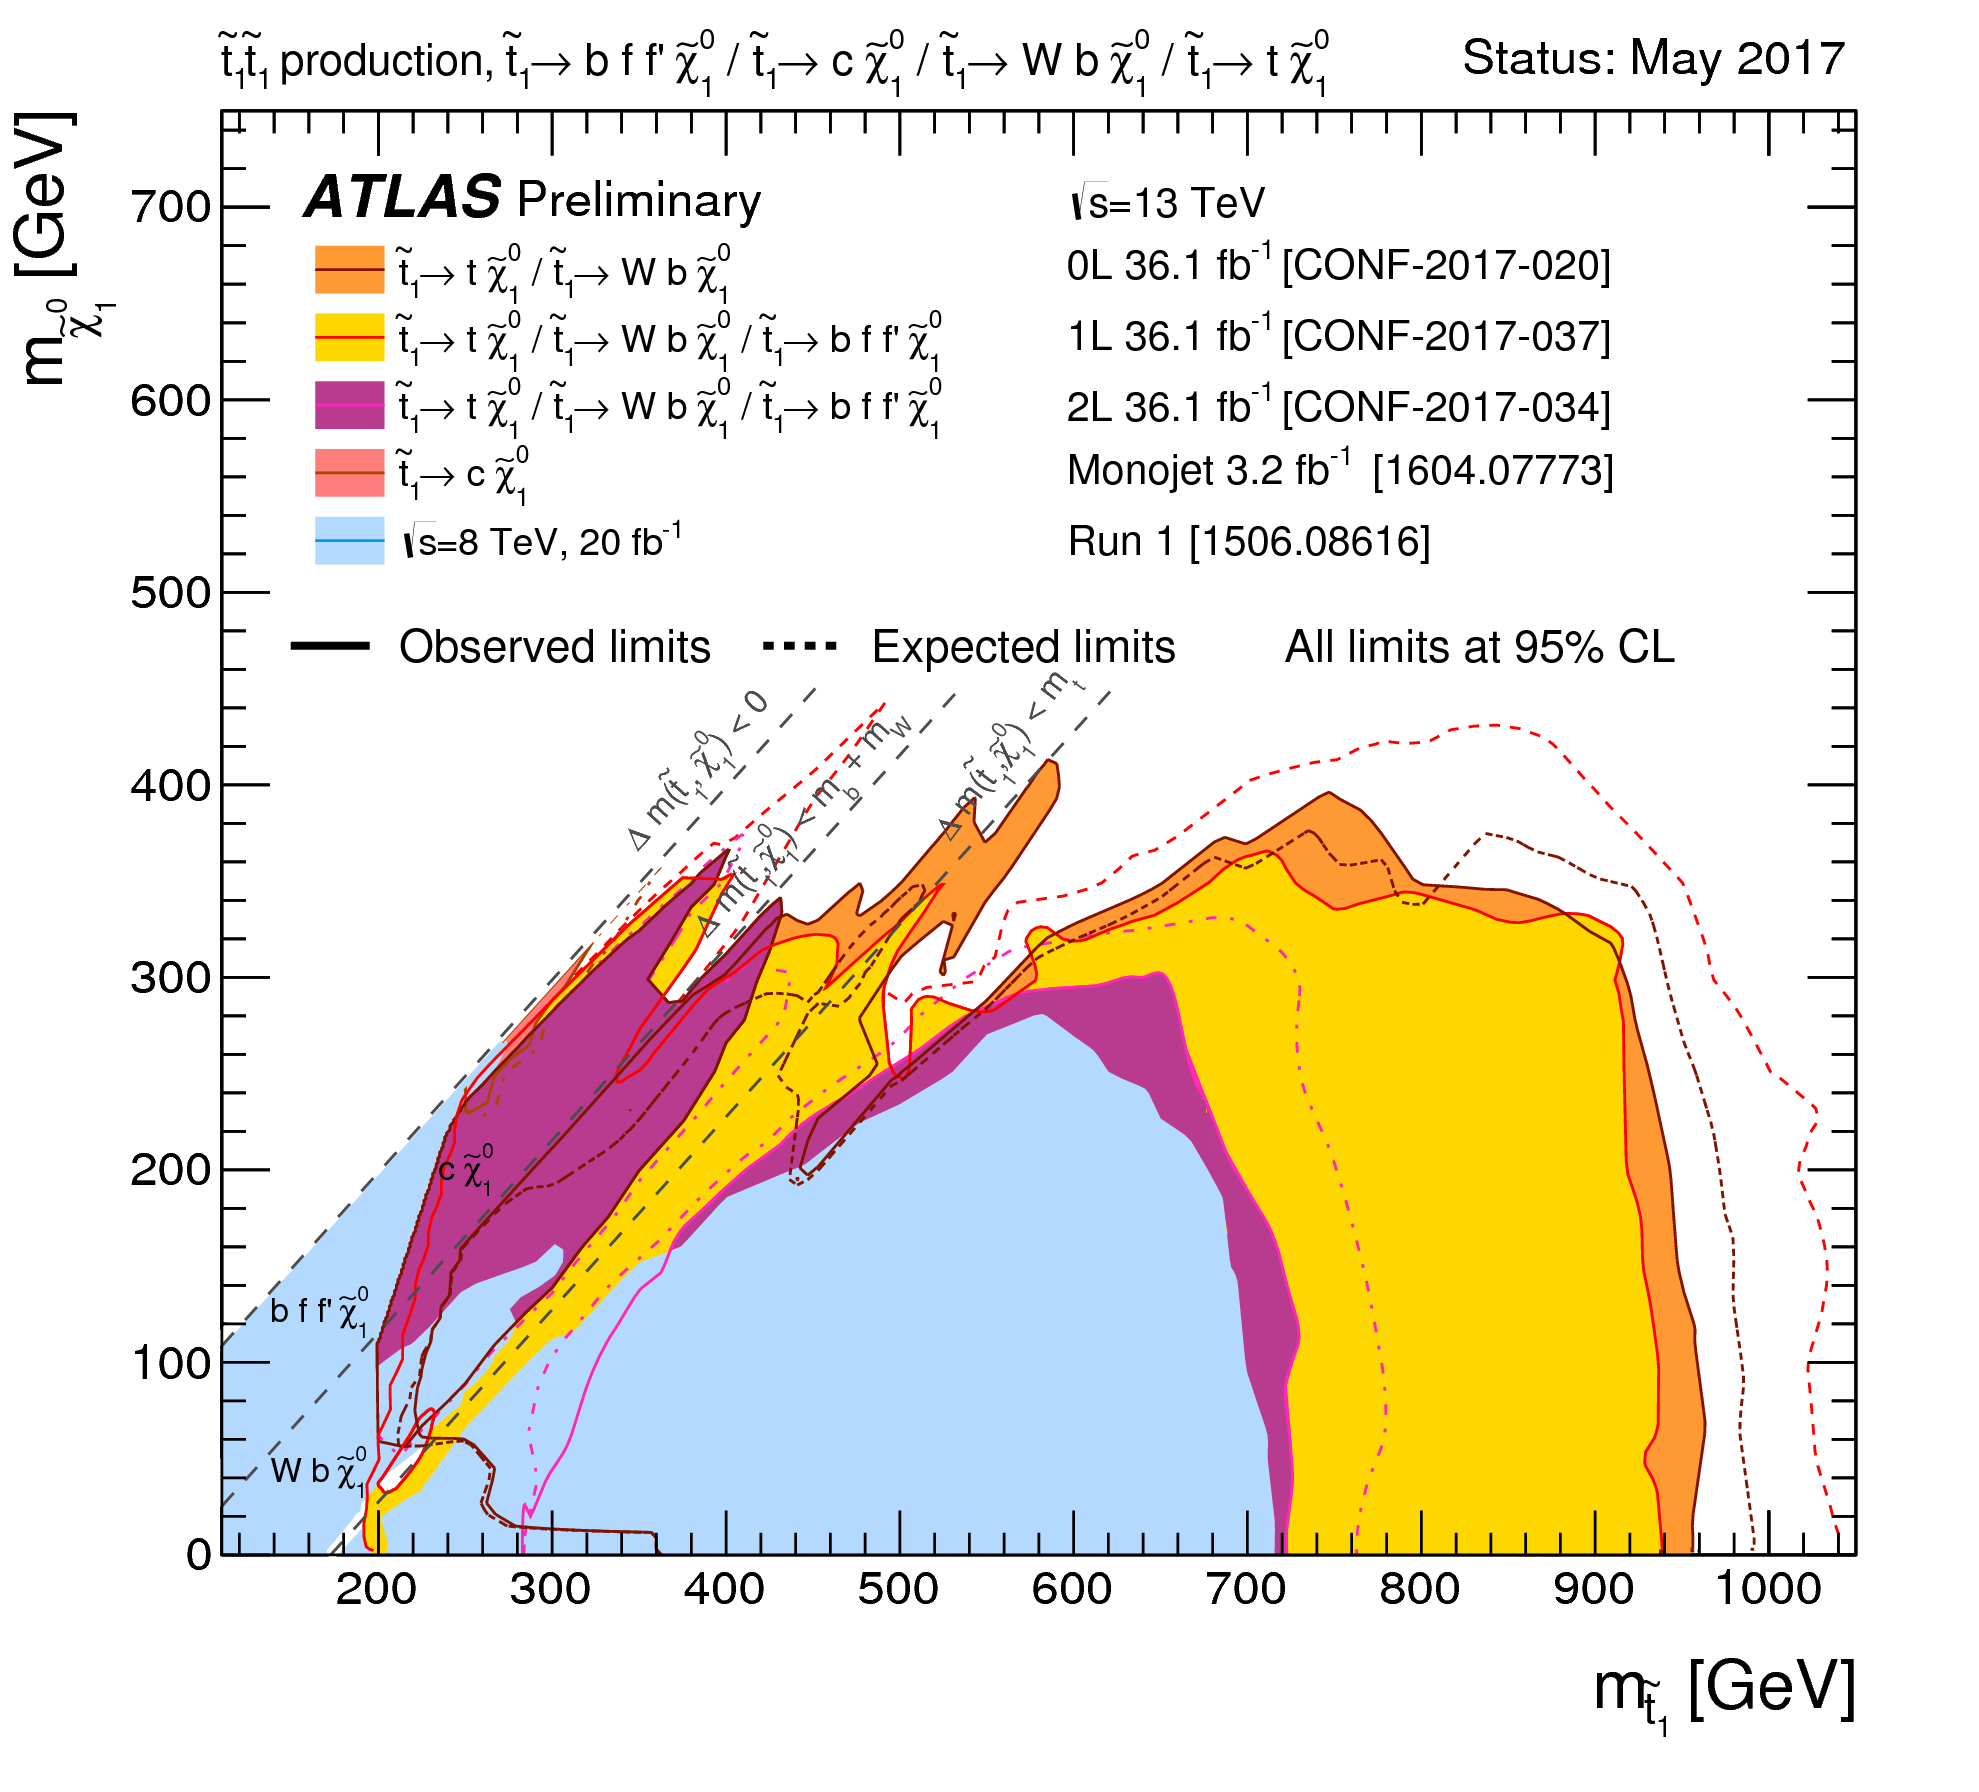
\includegraphics[width=0.7\linewidth]{{images/ATLAS_SUSY_Stop_tLSP}.png}
  \label{fig2.15}
\end{figure}

Whereas in the following figure there are the exclusion limits in ATLAS for p-p collisions at 13 TeV for the
channel invastiged in this project


 \begin{figure}[ht!]
  \centering
  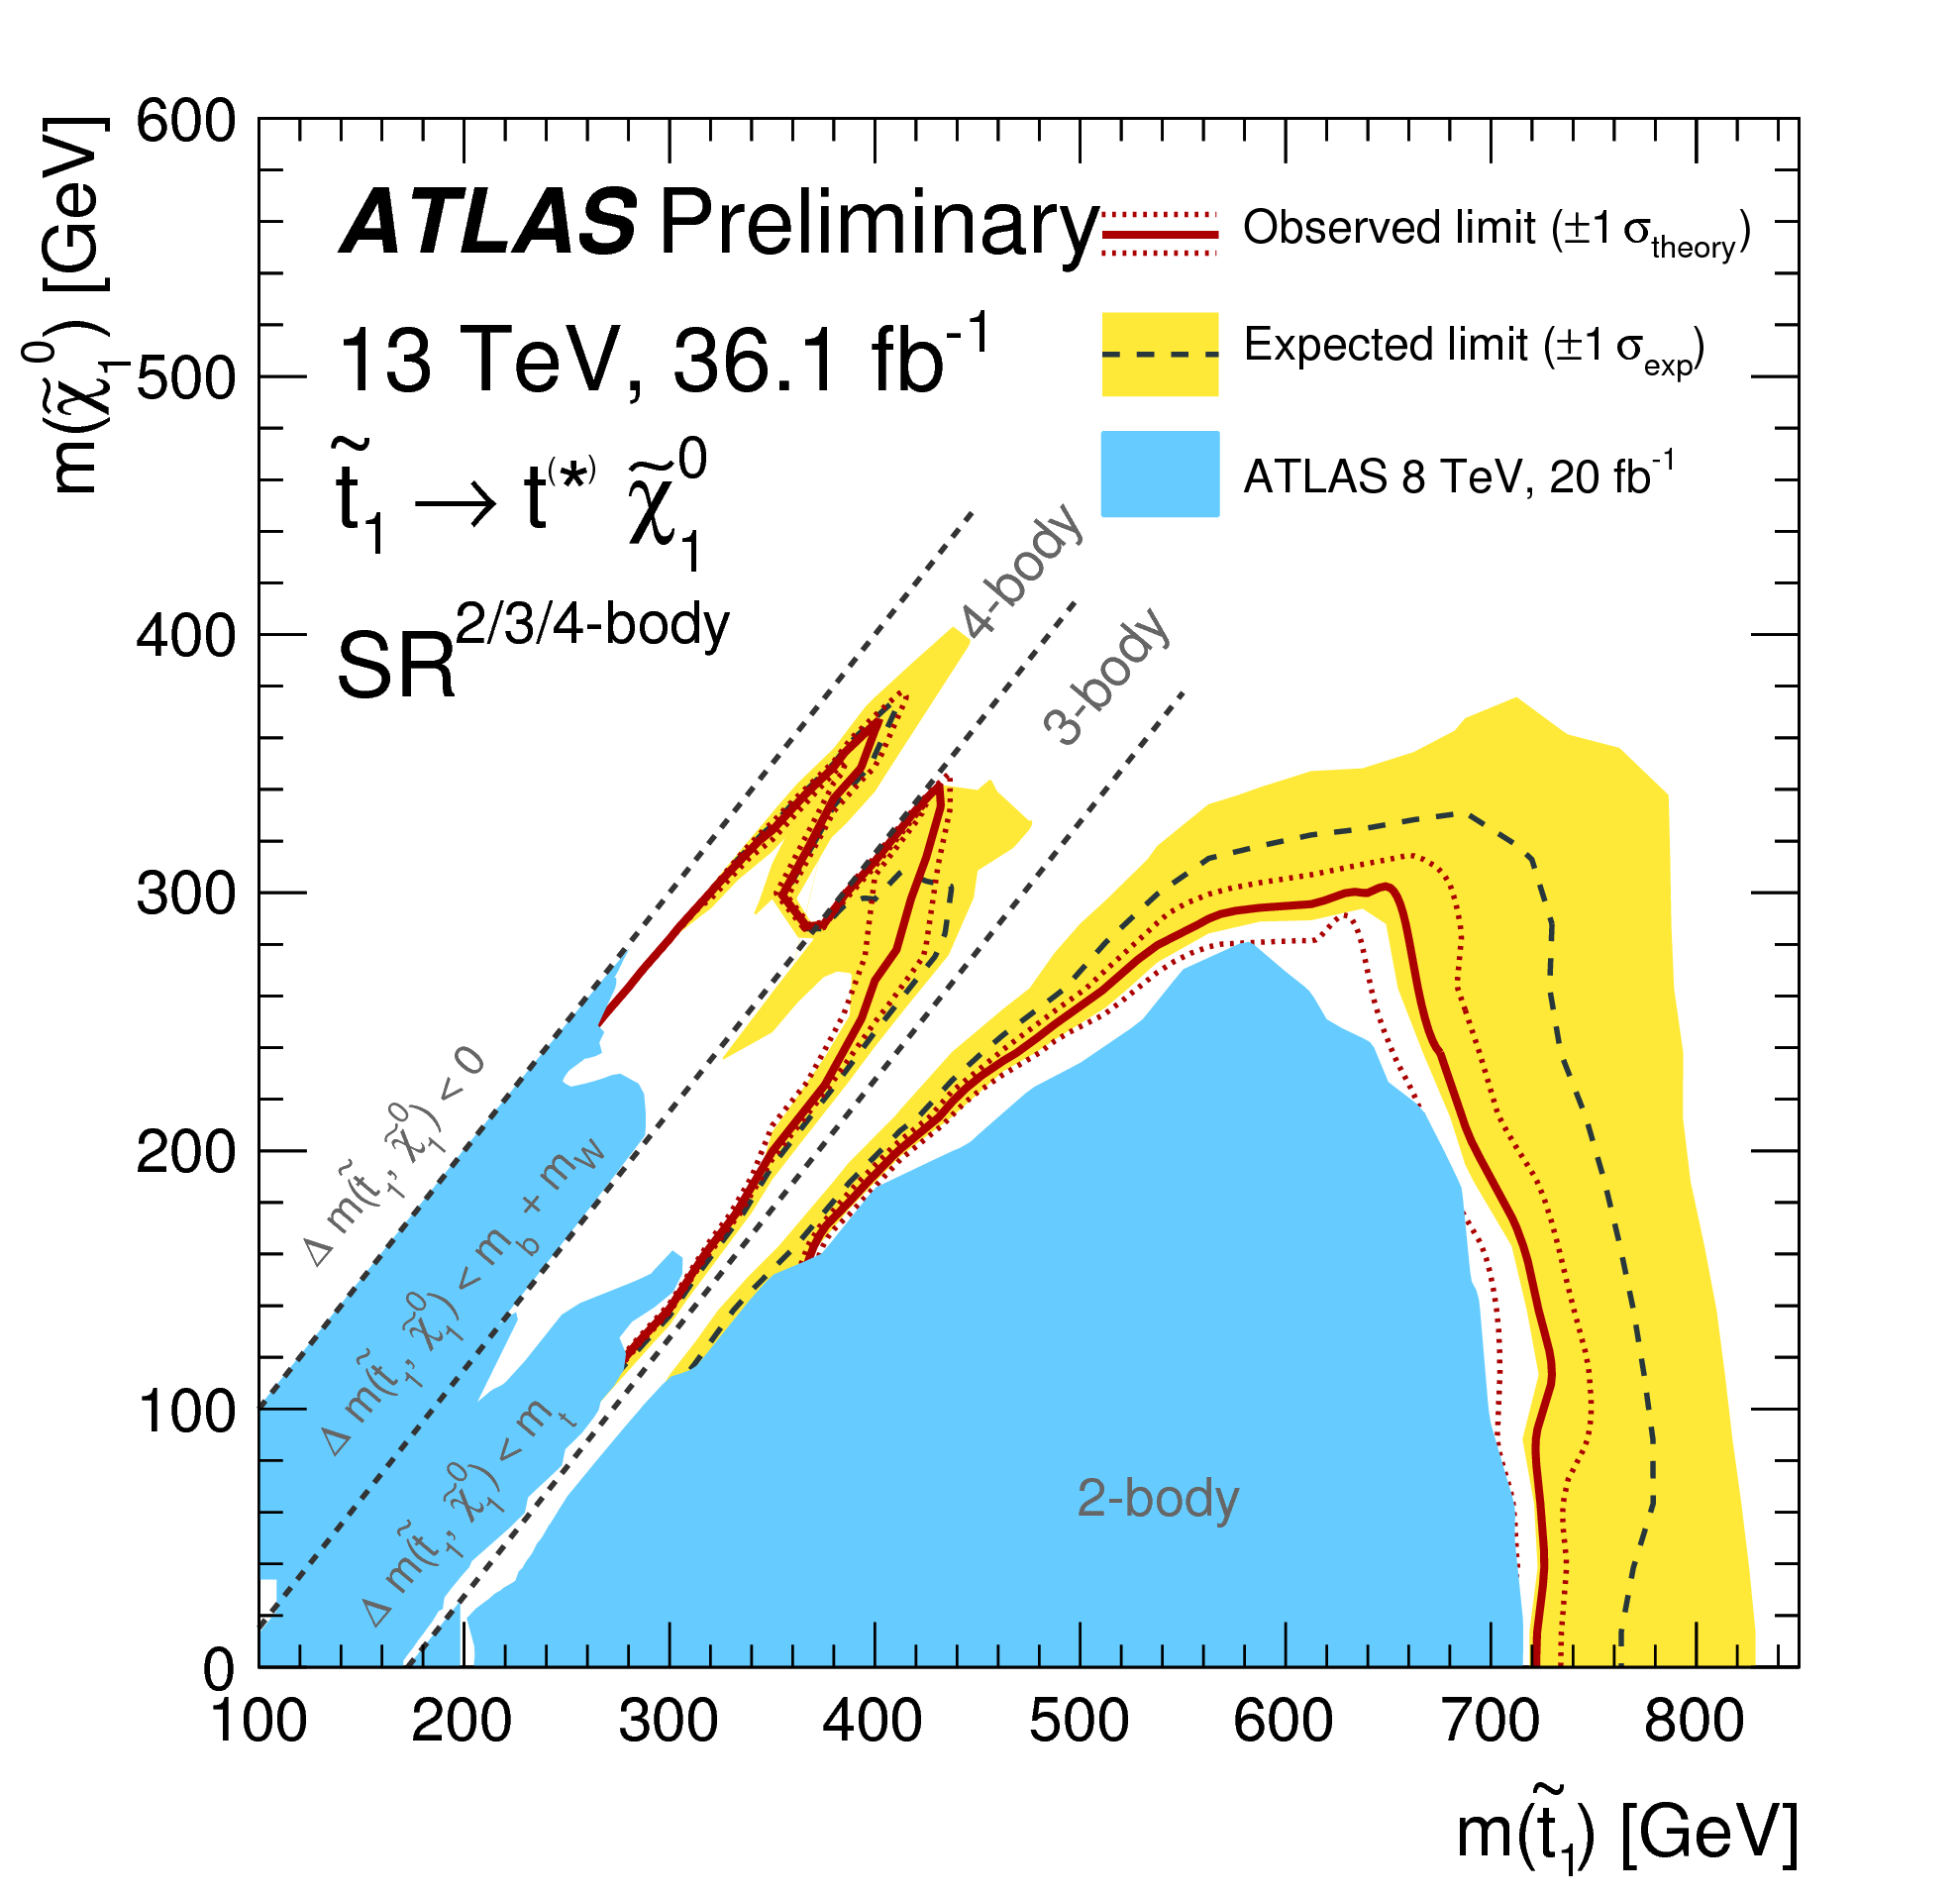
\includegraphics[width=0.7\linewidth, scale=5]{{images/fig_08}.png}
  \label{}
\end{figure}







\chapter{Methods}
\section{Introduction}

In this chapter I will describe the exact conditions and methods that were followed in this project for the 
calculation of the stop quark mass at CLIC Conceptual experiment.

I will invedtigate the production of a pair of stop quarks at $\surd s$ = 3 TeV and assumig an  integrated 
luminosity of $\mathcal{L}_{int}$ = 2000 fb$^{-1}$. The channel of interest is the following:

\begin{equation}
 e^{+} e^{+} \rightarrow \tilde{t} \tilde{\bar{t}} \rightarrow t\tilde{\chi}_{1}^{0} \bar{t}\tilde{\chi}_{1}^{0}
 \rightarrow W^{+}W^{-}b\bar{b} \tilde{\chi}_{1}^{0} \tilde{\chi}_{1}^{0}
\end{equation}

and for this model the mass of the top squark is $m_{\tilde{t}}$ = 844 GeV whereas the mass of the 
neutralino is $m_{\tilde{\chi}_{1}^{0}}$. This is not the only possible decay of a top squark but it is the
dominant one. In what follows I show the top three branching ratios of the top squark decay and two
of the corresponding Feynmann diagrams:

\begin{figure}[ht!]
  \raggedleft
  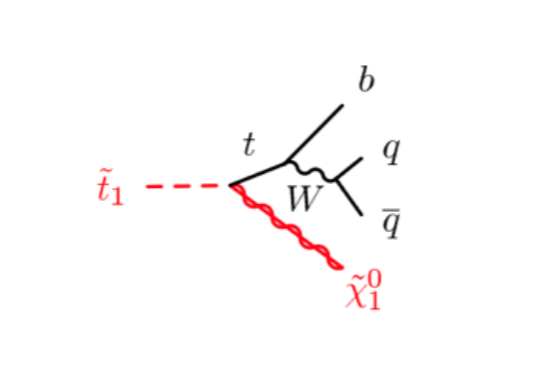
\includegraphics[width=0.4\linewidth]{{images/feyn1}.png}
  \hspace{\fill}
    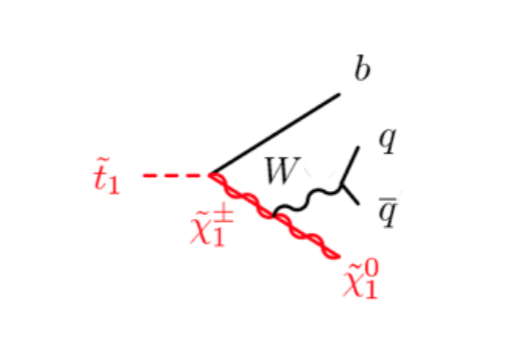
\includegraphics[width=0.4\linewidth]{{images/feyn2}.png}
  \label{}
\end{figure}


\newpage

\begin{enumerate}
 \item BR($\tilde{t}\rightarrow t \tilde{\chi}_{1}^{0}$) = 52.4 \%
 \item BR($\tilde{t}\rightarrow b \tilde{\chi}_{1}^{\pm}$) = 34.1 \%
 \item BR($\tilde{t}\rightarrow t \tilde{\chi}_{2}^{0}$) = 13.2 \%
 \end{enumerate}

As also the branching ratios for the decay of the W boson to either in a hadronic final state or in
a leptonic one are:

\begin{itemize}
 \item BR($W\rightarrow q\bar{q}$) = 67.8 \% 
 \item BR($W\rightarrow l\nu_{l}$) = 32.2 \%
\end{itemize}

In the following I summarise the possible decays of the stops indicating the branching pair fraction
for each one:

\begin{itemize}
 \item $e^{-}e^{+} \rightarrow \tilde{t}\tilde{\bar{t}} \rightarrow t \tilde{\chi}_{1}^{0}
 \chi^{\pm}_{1}b \rightarrow
 W^{+}W^{-} b \bar{b} \tilde{\chi}_{1}^{0}  \tilde{\chi}_{1}^{0}$ \quad (35.8\%)

 \item $e^{-}e^{+} \rightarrow \tilde{t}\tilde{\bar{t}} \rightarrow t\bar{t} \tilde{\chi}_{1}^{0}
 \tilde{\chi}^{0}_{1} \rightarrow
 W^{+}W^{-} b \bar{b} \tilde{\chi}_{1}^{0}  \tilde{\chi}_{1}^{0}$ \quad (27.4\%)

 \item $e^{-}e^{+} \rightarrow \tilde{t}\tilde{\bar{t}} \rightarrow t\bar{t} \tilde{\chi}_{1}^{0}
 \chi^{0}_{2} \rightarrow
 W^{+}W^{-} b \bar{b} \tilde{\chi}_{1}^{0}  \tilde{\chi}_{1}^{0}h$ \quad (13.7\%)
 
 \item $e^{-}e^{+} \rightarrow \tilde{t}\tilde{\bar{t}} \rightarrow b\bar{b} \chi_{1}^{+}
 \chi^{-}_{1} \rightarrow
 W^{+}W^{-} b \bar{b} \tilde{\chi}_{1}^{0}  \tilde{\chi}_{1}^{0}$ \quad (11.6\%)
 
 \item $e^{-}e^{+} \rightarrow \tilde{t}\tilde{\bar{t}} \rightarrow t \tilde{\chi}_{2}^{0}
 \chi^{\pm}_{1}b \rightarrow
 W^{+}W^{-} b \bar{b} \tilde{\chi}_{1}^{0}  \tilde{\chi}_{1}^{0}h$ \quad (9\%)
 
 \end{itemize}


\newpage

\section{Calculation of SUSY particle masses}

There are various ways that have been developed for the calculation of the squark masses at electron-positron
linear colliders. In this chapter I present one that will not be used in my analysis but sketch the potencial
and thus the importance of the aforementioned colliders regarding these kind of calculations.

The main topologies that are considered are those that the gluino is heavier than the squarks and thus the 
dominant decaying channel is:

\begin{equation}
 e^{-}e^{+} \rightarrow \tilde{q} \tilde{\bar{q}} \rightarrow q\bar{q}\chi_{1}^{0}\chi_{1}^{0}
\end{equation}

It needs to be mentioned that a powerfull advantage of the CLIC experiment is the possibility of achieving 
polarisation up to 80$\%$ helping to reduce the WW background and the ability to create right or left squarks
depending on the needs of the physical analysis.

\subsection{Modified Invariant Mass}

This technique has been developed initially for LHC experiment where the p-p collision energy is not known.
The calculation was achieved by creating the variable $M_{C}$ which is related to the standard 
invariant mass but it's invariance comes from contra linear boosts of equal magnitude. The squark mass is given
by:

\begin{equation}
 m_{\tilde{q}}=\frac{1}{2} \big(M_{C}^{max} + \sqrt{(M_{C}^{max})^{2} + 4m_{\chi}^{2}} \big)
\end{equation}

where 

\begin{equation}
 M_{C}^{2}=2(E_{q,1}E_{q,2}+\vec{p}_{q,1}\vec{p}_{q,2})
\end{equation}

and

\begin{equation}
 M_{C}^{max}=\frac{m^{2}_{\tilde{q}}-m^{2}_{\chi}}{m_{\tilde{q}}}
\end{equation}

The power off this kind of calculation comes from the fact that no knowledge for the exact center of mass 
energy is needed (In comparison with the first method described in~\cite{simon2010techniques}), something that is not purely known since the effects of initial state radiation and
the Beamstrahlung can distort it significantly resulting to even bigger uncertainties. Note that this method 
assumes that the mass of the neutralino is known and that the quark is massless. 

\section{Minimisaton of $\chi^{2}$ Method}

In this chapter I describe the procedure that I followed until the calculation of the top squark mass. 
This involved the vertex finding, the jet clustering, the flavourtagging and the calculation of the $\chi^{2}$
for each top squark mass.

\subsection{Vertex Finding}

For the needs of this projecct I used the package of LCFIplus which is an improved software of the already 
existing one LCFIVertex. The important difference between the  two is that LCFIplus employs the vertex finding 
befere the jet clustering (in comparison to LCFIVertex which follows the exact oposite procedure) with the 
goal to protect the secondadry vertices from breaking up and grouped into different jets~\cite{suehara2016lcfiplus}.
This is an important step towards better performance since the Bottom jets can be identified from their 
sufficiently large distance between the primary vertex and their decay vertex. Additionally, the importance
of this step to be performed before jet clustering, is that hadrons that contain bottom or charm quarks 
have sizeable lifetimes and they can be measured Inside the detector.


That said, the vertex finding was the first step towards obtaining the final data for analysis.

\subsection{Jet Clustering}

Jets are an indespensible part of high energy physics. They come from the manifestation of strong nuclear
as free quarks or gluons hadronize. They are visual structures that are measured in the detectors and they
serve the need of approaching the initial parton that they originated. Throught the years various algorithms 
have been developed for the clustering of such objects differing in the way that the approach suchh procedure.
Two of the most famous are the sequential recombination algorithms and cone algorithms. In this projecct I use
the a sequential recombination algorithm, the $k_{t}$ algorithm which is a longitudinaly invariant algorithm
firstly designed for hadron colliders.

The $k_{t}$ involves a measure of distance $d_{ij}$ for all the pair of particles $i,j$:

\begin{equation}
 d_{ij}=d_{ji}=min(p_{Ti}^{2},p_{Tj}^{2})\frac{\Delta R^{2}_{ij}}{R^{2}}
\end{equation}


where $p_{Ti}$ is the transverse momentum of $i^{th}$ particle with respect to beam direction and 
$\Delta R^{2}_{ij}=(y_{i}-y_{j})^{2}+(\phi_{i}-\phi_{j})^{2}$ with $y$ being the rapitdity, $\phi$ being
the azimuth angle and R the jet radius fixed in this project as $R=0.7$.

The basic idea behind this algorithm is that it calculates the $d_{ij}$ with the smallest value and then it 
"merges" the $i,j$ into a single object with momentum $p_{i}+p_{j}$. This procedure is repeated until the quantity
$d_{ij}$ is above some threshold and all the particles that are left are the event's jet
~\cite{cacciari2012fastjet}.

\subsection{Flavour Tagging}




\chapter{Results and Analysis}

This section should detail the obtained results in a clear,
easy-to-follow manner. It is important to make clear what are original
results and what are repeats of previous calculations or computations.
Remember that long tables of numbers are just as boring to read as
they are to type-in!

Use graphs to present your results wherever practicable.

Results or computations should be presented with uncertainties
(errors), both statistical and systematic where applicable.

Be selective in what you include: half a dozen \emph{e.g.}~tables that
contain wrong data you collected while you forgot to switch on the
computer are not relevant and may mask the correct results.


\section{Some results}
Here are some results.

\subsection{More results}
When showing results you are likely to use tables and graphs. You can
create tables easily in \LaTeX.

\begin{table}[h]
\begin{center}
\begin{tabular}{||l|c|l||}
\hline
\textbf{File names} & \textbf{Satellite} & \textbf{Resolution}\\
\hline
  worldr            &  Meteosat          &   5km\\
  worldg            &  Meteosat          &   5km\\
  worldb            &  Meteosat          &   5km\\
\hline
\end{tabular}
\end{center}
\caption{This is a simple table. More complicated tables can have
headings which pass over more than one column}
\label{simple_table}
\end{table}

If you want to produce fancier tables than shown in Table \ref{simple_table}
refer to the \LaTeX\ manual or ask Google.

One of the simplest ways to produce simple graphs is to use gnuplot
which produces \LaTeX\  output. Graph~(\ref{fig:gnu}) was produced using
gnuplot with output designated as \LaTeX\  so that a \LaTeX\  output file is
produced which you can include directly or keep separate and refer to
using the \emph{include} command.

Another approach is to draw simple figures using \emph{xfig} which allows
you to export diagrams in \LaTeX\  picture format so that the diagram can
be included directly.

Perhaps the most robust way to include graphs is to convert them to
PostScript or PDF and include them in the same was as was done in
Figure~\ref{fig:eucrest} for the University Crest. You can usually do
this with most packages, including Microsoft ones; one trick for
producing PostScript is to print to a dummy PostScript printer.

% in practice you would probably keep this in a separate file and use
% the \include{filename} command to insert it here.

\begin{figure}
% GNUPLOT: LaTeX picture
\setlength{\unitlength}{0.240900pt}
\ifx\plotpoint\undefined\newsavebox{\plotpoint}\fi
\sbox{\plotpoint}{\rule[-0.200pt]{0.400pt}{0.400pt}}%
\begin{picture}(1500,1200)(0,0)
\font\gnuplot=cmr10 at 10pt
\gnuplot
\sbox{\plotpoint}{\rule[-0.200pt]{0.400pt}{0.400pt}}%
\put(220.0,113.0){\rule[-0.200pt]{292.934pt}{0.400pt}}
\put(220.0,113.0){\rule[-0.200pt]{0.400pt}{245.477pt}}
\put(220.0,113.0){\rule[-0.200pt]{4.818pt}{0.400pt}}
\put(198,113){\makebox(0,0)[r]{$0$}}
\put(1416.0,113.0){\rule[-0.200pt]{4.818pt}{0.400pt}}
\put(220.0,317.0){\rule[-0.200pt]{4.818pt}{0.400pt}}
\put(198,317){\makebox(0,0)[r]{$0.2$}}
\put(1416.0,317.0){\rule[-0.200pt]{4.818pt}{0.400pt}}
\put(220.0,521.0){\rule[-0.200pt]{4.818pt}{0.400pt}}
\put(198,521){\makebox(0,0)[r]{$0.4$}}
\put(1416.0,521.0){\rule[-0.200pt]{4.818pt}{0.400pt}}
\put(220.0,724.0){\rule[-0.200pt]{4.818pt}{0.400pt}}
\put(198,724){\makebox(0,0)[r]{$0.6$}}
\put(1416.0,724.0){\rule[-0.200pt]{4.818pt}{0.400pt}}
\put(220.0,928.0){\rule[-0.200pt]{4.818pt}{0.400pt}}
\put(198,928){\makebox(0,0)[r]{$0.8$}}
\put(1416.0,928.0){\rule[-0.200pt]{4.818pt}{0.400pt}}
\put(220.0,1132.0){\rule[-0.200pt]{4.818pt}{0.400pt}}
\put(198,1132){\makebox(0,0)[r]{$1$}}
\put(1416.0,1132.0){\rule[-0.200pt]{4.818pt}{0.400pt}}
\put(220.0,113.0){\rule[-0.200pt]{0.400pt}{4.818pt}}
\put(220,68){\makebox(0,0){$0$}}
\put(220.0,1112.0){\rule[-0.200pt]{0.400pt}{4.818pt}}
\put(414.0,113.0){\rule[-0.200pt]{0.400pt}{4.818pt}}
\put(414,68){\makebox(0,0){$1$}}
\put(414.0,1112.0){\rule[-0.200pt]{0.400pt}{4.818pt}}
\put(607.0,113.0){\rule[-0.200pt]{0.400pt}{4.818pt}}
\put(607,68){\makebox(0,0){$2$}}
\put(607.0,1112.0){\rule[-0.200pt]{0.400pt}{4.818pt}}
\put(801.0,113.0){\rule[-0.200pt]{0.400pt}{4.818pt}}
\put(801,68){\makebox(0,0){$3$}}
\put(801.0,1112.0){\rule[-0.200pt]{0.400pt}{4.818pt}}
\put(995.0,113.0){\rule[-0.200pt]{0.400pt}{4.818pt}}
\put(995,68){\makebox(0,0){$4$}}
\put(995.0,1112.0){\rule[-0.200pt]{0.400pt}{4.818pt}}
\put(1188.0,113.0){\rule[-0.200pt]{0.400pt}{4.818pt}}
\put(1188,68){\makebox(0,0){$5$}}
\put(1188.0,1112.0){\rule[-0.200pt]{0.400pt}{4.818pt}}
\put(1382.0,113.0){\rule[-0.200pt]{0.400pt}{4.818pt}}
\put(1382,68){\makebox(0,0){$6$}}
\put(1382.0,1112.0){\rule[-0.200pt]{0.400pt}{4.818pt}}
\put(220.0,113.0){\rule[-0.200pt]{292.934pt}{0.400pt}}
\put(1436.0,113.0){\rule[-0.200pt]{0.400pt}{245.477pt}}
\put(220.0,1132.0){\rule[-0.200pt]{292.934pt}{0.400pt}}
\put(45,622){\makebox(0,0){\shortstack{This is\\the\\$y$ axis}}}
\put(828,23){\makebox(0,0){This is the $x$ axis}}
\put(828,1177){\makebox(0,0){This is a plot of $y=sin(x)$}}
\put(220.0,113.0){\rule[-0.200pt]{0.400pt}{245.477pt}}
\sbox{\plotpoint}{\rule[-0.500pt]{1.000pt}{1.000pt}}%
\put(1306,1067){\makebox(0,0)[r]{sin(x)}}
\multiput(1328,1067)(20.756,0.000){4}{\usebox{\plotpoint}}
\put(1394,1067){\usebox{\plotpoint}}
\put(220,113){\usebox{\plotpoint}}
\multiput(220,113)(3.768,20.411){4}{\usebox{\plotpoint}}
\multiput(232,178)(4.132,20.340){3}{\usebox{\plotpoint}}
\multiput(245,242)(3.825,20.400){3}{\usebox{\plotpoint}}
\multiput(257,306)(3.884,20.389){3}{\usebox{\plotpoint}}
\multiput(269,369)(3.944,20.377){3}{\usebox{\plotpoint}}
\multiput(281,431)(4.326,20.300){3}{\usebox{\plotpoint}}
\multiput(294,492)(4.137,20.339){3}{\usebox{\plotpoint}}
\multiput(306,551)(4.276,20.310){3}{\usebox{\plotpoint}}
\multiput(318,608)(4.693,20.218){3}{\usebox{\plotpoint}}
\multiput(331,664)(4.583,20.243){2}{\usebox{\plotpoint}}
\multiput(343,717)(4.754,20.204){3}{\usebox{\plotpoint}}
\multiput(355,768)(5.034,20.136){2}{\usebox{\plotpoint}}
\multiput(367,816)(5.760,19.940){2}{\usebox{\plotpoint}}
\multiput(380,861)(5.579,19.992){3}{\usebox{\plotpoint}}
\put(398.00,923.50){\usebox{\plotpoint}}
\multiput(404,943)(7.049,19.522){2}{\usebox{\plotpoint}}
\multiput(417,979)(7.288,19.434){2}{\usebox{\plotpoint}}
\put(433.18,1021.10){\usebox{\plotpoint}}
\multiput(441,1040)(8.982,18.712){2}{\usebox{\plotpoint}}
\put(460.41,1076.97){\usebox{\plotpoint}}
\put(471.84,1094.28){\usebox{\plotpoint}}
\put(484.84,1110.41){\usebox{\plotpoint}}
\put(500.42,1124.01){\usebox{\plotpoint}}
\multiput(503,1126)(19.159,7.983){0}{\usebox{\plotpoint}}
\put(519.48,1131.37){\usebox{\plotpoint}}
\multiput(527,1132)(20.136,-5.034){0}{\usebox{\plotpoint}}
\put(539.74,1128.60){\usebox{\plotpoint}}
\put(557.04,1117.38){\usebox{\plotpoint}}
\put(570.79,1101.95){\usebox{\plotpoint}}
\put(582.44,1084.80){\usebox{\plotpoint}}
\put(593.09,1066.99){\usebox{\plotpoint}}
\multiput(601,1053)(8.430,-18.967){2}{\usebox{\plotpoint}}
\put(619.18,1010.54){\usebox{\plotpoint}}
\multiput(625,996)(7.413,-19.387){2}{\usebox{\plotpoint}}
\multiput(638,962)(6.403,-19.743){2}{\usebox{\plotpoint}}
\multiput(650,925)(5.830,-19.920){2}{\usebox{\plotpoint}}
\multiput(662,884)(5.461,-20.024){2}{\usebox{\plotpoint}}
\multiput(674,840)(5.533,-20.004){2}{\usebox{\plotpoint}}
\multiput(687,793)(4.937,-20.160){3}{\usebox{\plotpoint}}
\multiput(699,744)(4.667,-20.224){2}{\usebox{\plotpoint}}
\multiput(711,692)(4.858,-20.179){3}{\usebox{\plotpoint}}
\multiput(724,638)(4.276,-20.310){3}{\usebox{\plotpoint}}
\multiput(736,581)(4.205,-20.325){3}{\usebox{\plotpoint}}
\multiput(748,523)(4.070,-20.352){3}{\usebox{\plotpoint}}
\multiput(760,463)(4.326,-20.300){3}{\usebox{\plotpoint}}
\multiput(773,402)(3.884,-20.389){3}{\usebox{\plotpoint}}
\multiput(785,339)(3.884,-20.389){3}{\usebox{\plotpoint}}
\multiput(797,276)(4.070,-20.352){3}{\usebox{\plotpoint}}
\multiput(810,211)(3.825,-20.400){3}{\usebox{\plotpoint}}
\multiput(822,147)(3.607,-20.440){2}{\usebox{\plotpoint}}
\put(828,113){\usebox{\plotpoint}}
\end{picture}
\caption{Simple Gnuplot example}
\label{fig:gnu}
\end{figure}

\section{Discussion of your results}

This section should give a picture of what you have taken out of your
project and how you can put it into context.

This section should summarise the results obtained, detail conclusions
reached, suggest future work, and changes that you would make if you
repeated the project.

\chapter{Conclusions}

This is the place to put your conclusions about your work. You can
split it into different sections if appropriate. You may want to include
a section of future work which could be carried out to continue your
research.

The conclusion section should be at least one page long, preferably 2
pages, but not much longer.

\appendix
% the appendix command just changes heading styles for appendices.

\chapter{Stuff that's too detailed}

Appendices should contain all the material which is considered too
detailed to be included in the main body of the text, but which is
important enough to be included in the thesis.

Perhaps this is a good place to mention \BibTeX.

You can do references in the simple way explained in the introduction,
or you can use \BibTeX.


\section{\BibTeX}
\label{sec:bibtex}

It is convenient to use \BibTeX\ to compile your bibliography.  First
you need to create a .bib file e.g.  you may call it ref.bib Then you
can put all your references into the file with entries such as
\begin{verbatim}
@Book{ob:bornwolf,
     author = "Born, M and Wolf, E",
     title  = "Principles of Optics",
     publisher = "Cambridge University Press",
     year = 1999,
     edition = {7th},
}

@Article{jr:ashkin,
Author = {A. Ashkin and J.M. Dziedzic and J.E. Bjorkholm and S. Chu},
Title = "Observation of a single beam gradient force optical tap for 
dielectric particles",
Journal = "Optics Letters",
Volume = 11,
Pages = "288-290",
Year = 1986}

@INPROCEEDINGS{seger,
 author = {J. Seger and H.J. Brockman},
 title = {What is bet-hedging?},
 editors={P.H. Harvey and L. Partridge},
 booktitle = {Oxford Surveys in Evolutionary Biology},
 year={1987},
 page={18},
 publisher={Oxford University Press},
 place={Oxford}}
\end{verbatim}
for a book, an article in a journal or an article in a proceedings volume
respectively.

Inside your \LaTeX\ file
you should include 
\begin{verbatim}
\bibliographystyle{unsrt}                      
and
\bibliography{ref}
\end{verbatim}
The first command determines the reference style, here plain and 
unsorted. With this referencing style 
a numerical referencing system (which is now the most
common in physics literature) is used and the numbering of references
will be the order in which they appear in the document. Alternatively, 
you could use
a customised `style file' but there is no real need.  The second
command just inputs your .bib file Note that only the references cited
in the text will appear in the bibliography so you can have spare
references in your .bib file.


You use the name you have given to an entry (e.g.
for the book example above the name is ob:bornwolf)
to cite the relevant article
by using the cite command in your \LaTeX\ file e.g. \cite{ob:bornwolf}



\section{Producing your documents using \texttt{pdflatex}}

To use pdflatex your figures need to be in pdf format.  You can convert almost any image file to pdf using \texttt{convert}.  e.g. \texttt{convert myfigure.png myfigure.pdf}.

The first time you should type:
\begin{verbatim}
  pdflatex ProjectReport
  bibtex ProjectReport
  pdflatex ProjectReport
  pdflatex ProjectReport
\end{verbatim} 
This first time you run\texttt{pdflatex} it will produce a
\texttt{ProjectReport.aux}.  The \BibTeX\ command reads in the
bibliography file and makes the files \texttt{ProjectReport.bbl} and
\texttt{ProjectReport.blg} files.  These files are read in the next
\texttt{pdflatex} command, but you'll still have ``undefined
cross-reference'' errors which are sorted out by the last
\texttt{pdflatex} command.

Subsequently, you should only need to do one (or two)
\texttt{pdflatex}s, or \texttt{pdfbibtex} followed by
\texttt{pdflatex} twice if you change any references.

\vspace{5mm} You may also use plain \texttt{latex} instead of
\texttt{pdflatex}.  This requires you to use postscript graphics
instead of pdf.




\chapter{Stuff that won't be read by anyone}

Some people include in their thesis a lot of detail, particularly lots
of tables containing raw results, figures of intermediate results, or
computer code which no-one will ever read. You should be careful that
anything like this you include should contain some element of
uniqueness which justifies its inclusion.


\newpage

\bibliographystyle{unsrt}
\bibliography{MSc_dissertation}


\end{document}

